\clearpage
\section{项目图片}

以下六图均取自当前作品的实际运行界面或演示视频，已裁到与说明相关的区域。它们不是界面设计稿，也不使用整屏缩小来凑图。截图中的题目和卡片来自自写教学样例，不包含真实学生资料。图片用于核对交互与结果形态，具体质量结论仍以第 3 节的测试和评测口径为准。

\subsection{首次启动引导与知识卡片}

新手引导只覆盖上传、出题、批改和谱系四个入口。首次访问、桌面版首次启动、地址带 \env{?tour=1} 或用户主动点击顶栏入口时出现。关闭后写入本地完成标记，刷新不重复打断操作。引导的作用是缩短第一次使用时的寻找成本，不替代实际流程中的状态提示。

\begin{figure}[H]
\centering
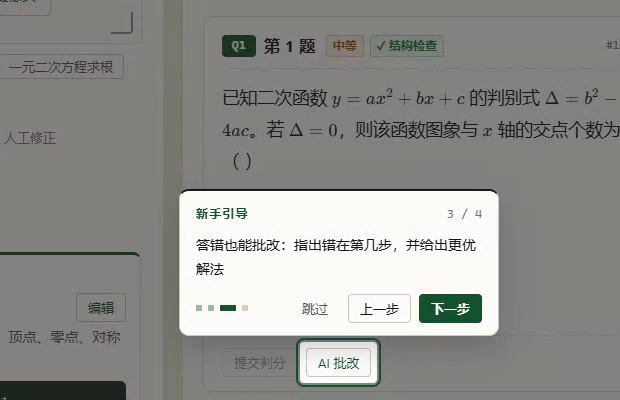
\includegraphics[width=0.58\textwidth,height=5.0cm,keepaspectratio]{img/c01.png}
\caption{四步新手引导中的批改版块。遮罩保留目标区域可见，说明分数、出错步骤和更优解法的入口。}
\label{fig:ui-tour}
\end{figure}

卡片区把模型结果保持为可编辑对象，而非只读摘要。标题、摘要、公式和正文均可修订，保存后当前列表就地更新，来源关系和创建时间不变。修改历史记录旧值与新值，刷新后仍可查看。这个入口位于识别和命题之间，使用户能够在错误进入练习前进行处理。

\begin{figure}[H]
\centering
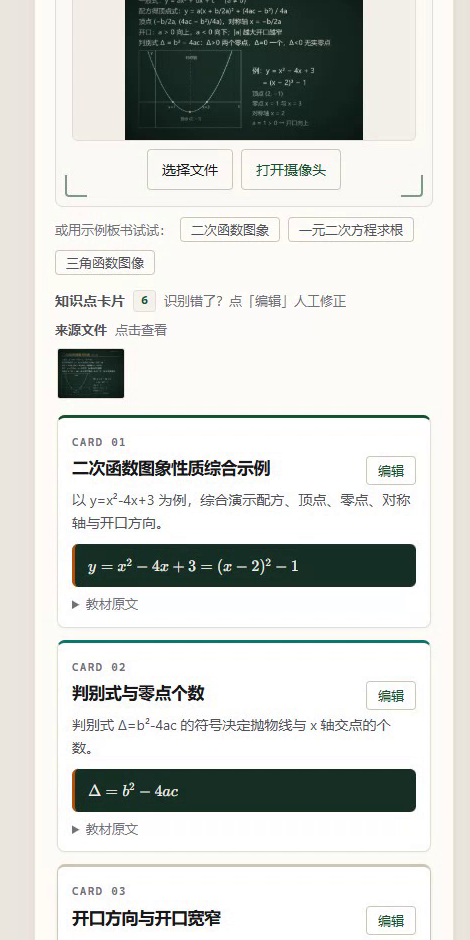
\includegraphics[height=7.7cm,keepaspectratio]{img/02-cards.png}
\caption{识别来源与知识卡片局部。卡片按字段展示，公式由 KaTeX 渲染，编辑入口用于人工修正与历史查看。}
\label{fig:ui-cards}
\end{figure}

\clearpage
\subsection{逐条出题、验算级别与分步批改}

出题结果按题逐条进入练习卷。卡片上的徽章区分“已验算”和“结构检查”，顶部汇总分别统计不同级别。题目进入列表不代表检查已经结束，质检事件继续更新状态。图中所示批次包含符号验算与结构检查两类结果，说明系统没有用同一“通过”标签掩盖检查深度。

\begin{figure}[H]
\centering
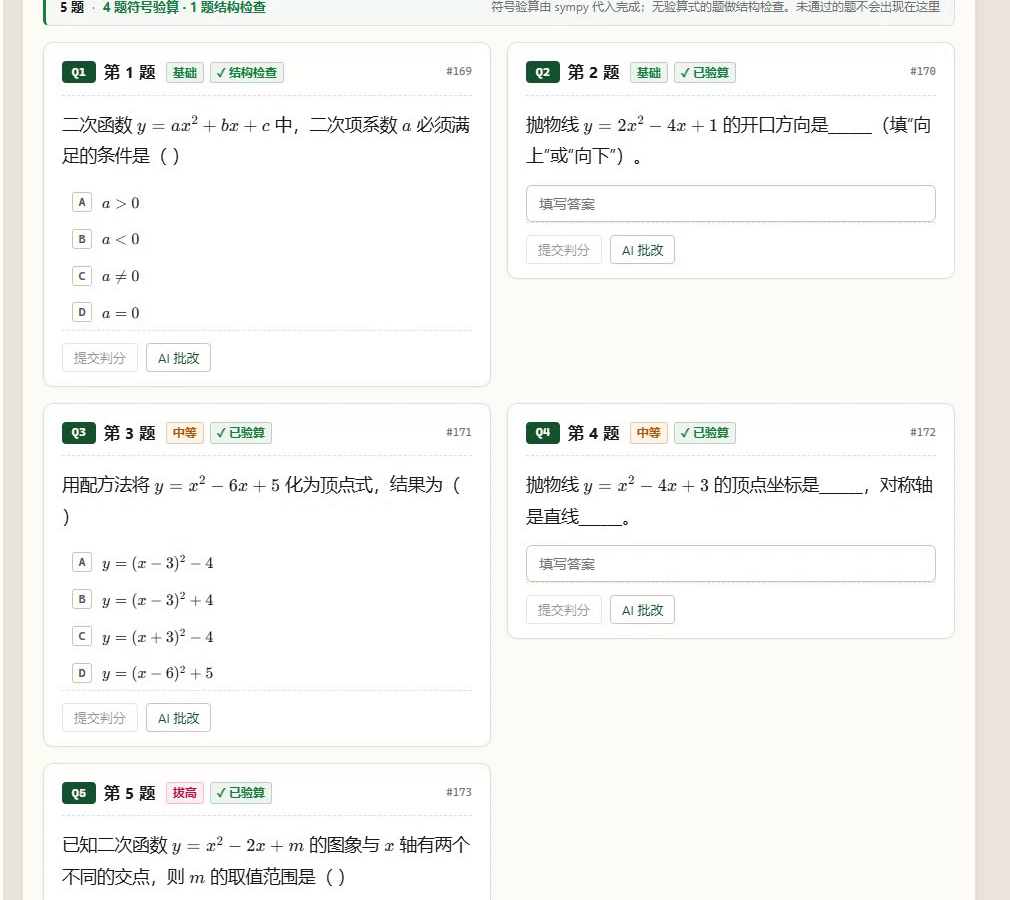
\includegraphics[width=0.69\textwidth,height=9.4cm,keepaspectratio]{img/c03.png}
\caption{命题结果与验收单局部。题目逐条出现，验算级别和批次汇总来自后端题目对象及结束事件。}
\label{fig:ui-questions}
\end{figure}

批改面板把分数与步骤诊断放在同一视图中。首个错误步骤被明确标出，后续区域给出原因和改进建议。分数环和步骤高亮由结构化结束事件驱动，连续评语由分片事件驱动，因此正文逐步出现时，步骤结论不会失去可核对性。mock 下只展示规则能够支持的诊断，不伪造学生方法归因。

\begin{figure}[H]
\centering
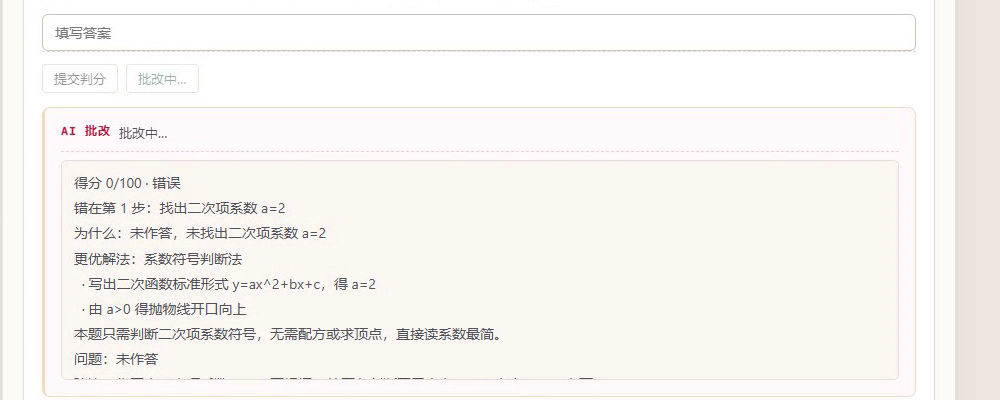
\includegraphics[width=0.96\textwidth,height=6.1cm,keepaspectratio]{img/c04.png}
\caption{AI 批改局部。示例定位到首个错误步骤，并给出错误原因、更优解法和后续建议。}
\label{fig:ui-review}
\end{figure}

\clearpage
\subsection{错题讲解函数图与知识谱系}

讲解图将抽象系数变成可拖动参数。当前二次函数模板固定观察范围，避免每次拖动都重新缩放坐标系。独立函数图入口允许输入受限表达式，解析失败时显示错误，不执行字符串代码。图像用于辅助理解，不代替步骤诊断，也不表示已经支持任意学科的可视化模板。

\begin{figure}[H]
\centering
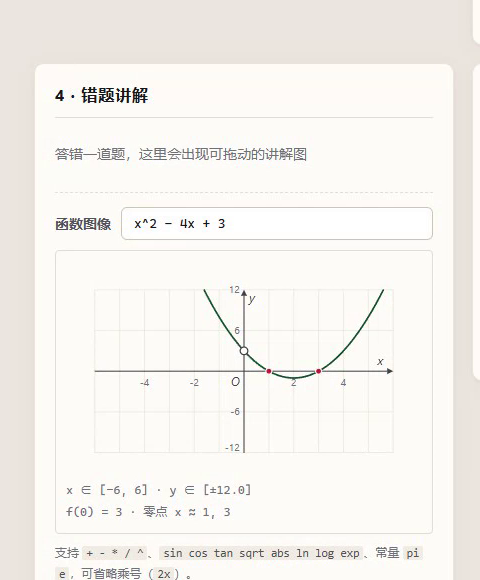
\includegraphics[height=9.5cm,keepaspectratio]{img/05-graph.png}
\caption{错题讲解与函数图局部。表达式、参数和图像保持同步，特殊点按可见范围绘制。}
\label{fig:ui-graph}
\end{figure}

知识谱系按共享标签建边，节点大小表示该卡片关联的出题量，颜色深浅表示被问次数，侧栏列出高频卡片。泛化程度过高的标签不用于建边，减少无意义的全连接。该图用于定位个人资料中的活跃主题，不作为学生掌握度评分。

\begin{figure}[H]
\centering
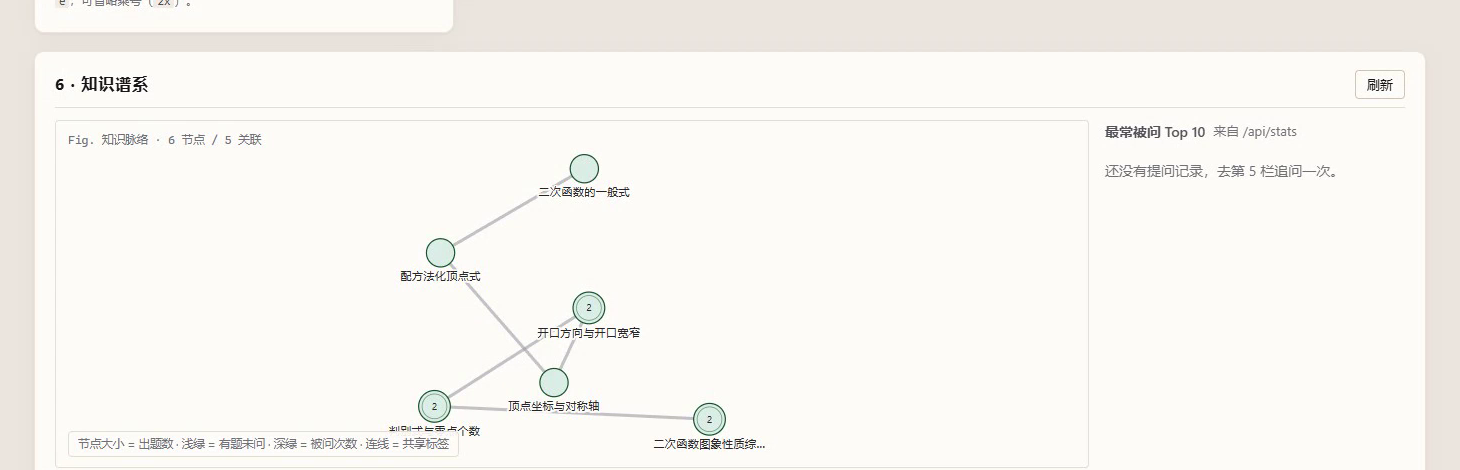
\includegraphics[width=0.97\textwidth,height=5.0cm,keepaspectratio]{img/c06.png}
\caption{知识谱系局部。节点、共享标签关系、原图入口与高频榜来自同一批本地卡片和计数。}
\label{fig:ui-lineage}
\end{figure}
